The recognition of an object in a scene with precision can be a trick problem to be solved, and to increase the experience with some virtual artifacts calls for a high level of localization accuracy.

This paper presents an approach based a pre-known 3d representation of the scene.

The real time reconstruction of the scene are fundamental to reduce the cumulative error added to the recognition added after each frame because of interest point recognition hardness caused by light variation, textures and other issues studied in this essay.
As proposed in \cite{ISMAR2012}

\begin{figure}[ht!]
\centering
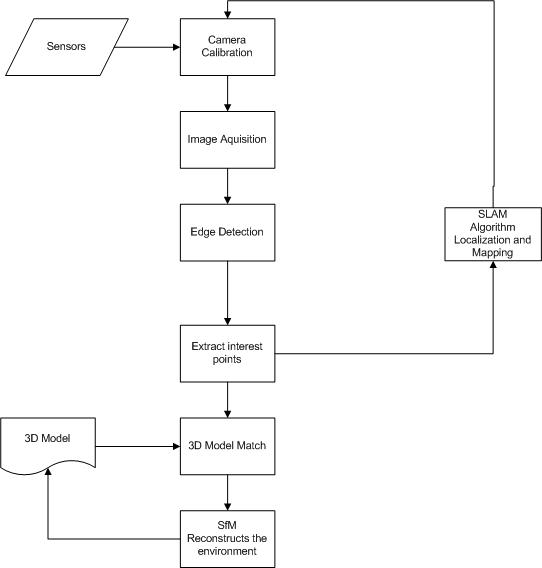
\includegraphics[width=90mm]{images/algorithm.jpg}
\caption{Algorithm Diagram}
\label{algorithm}
\end{figure}


\subsection{Camera Calibration}

\subsubsection{Error Reduction Approach}

\subsection{Image Acquisition}

\subsection{Edge Detection}

\subsection{Extract Interest Points}

\subsection{Model Match}

\subsubsection{Real Time Model Reconstruction}